%% =====================================================================
%% What a Tooth-Level Score Cannot Tell You:
%% Constant Baselines, External Validation and Domain Shift in
%% Automated Panoramic Dental Screening
%%
%% IEEE conference format (IEEEtran).
%% Authors intentionally set to "Unknown" pending author-order decision.
%%
%% REBUILT 28 August 2026. Every numeric claim in this file traces to a
%% saved artefact: outputs/*.json, models/<NN>_*/run_summary.txt, or a
%% recomputation recorded in docs/paper/REBUILD_AUDIT.md. Nothing is
%% estimated or recalled. The superseded first draft is preserved at
%% _repo_archive/paper_draft_v1_44percent_title/.
%%
%% Five defects corrected against the previous draft, each documented in
%% REBUILD_AUDIT.md Deliverable 3b:
%%   1. whole-system parameter count 25 M -> 83.6 M (counted from weights)
%%   2. VLM names "33B"/"8B" -> the released 32B-Instruct / 7B-Instruct
%%   3. blank-image control was overstated for the larger model
%%   4. isotonic calibration does NOT leave verdicts unchanged by nature
%%   5. the "no paper reports a baseline" claim was never counted
%%
%% REBUILT 11 October 2026 on the multi-corpus tooth detector, which became the
%% Stage-1 default that day by a decision against two pre-registered ablation
%% verdicts (RESULTS_LOG 2026-10-11f). Every pipeline number was re-measured with
%% both detectors on one machine -- outputs/stage1_switch/, RESULTS_LOG
%% 2026-10-11g to -j. The development-data headline changed with the detector:
%% the pipeline now scores above the image-blind constant on DENTEX and is still
%% not separable from it on external data. docs/paper/SUBMISSION_TODO.md Sec 1.
%% =====================================================================
\documentclass[conference]{IEEEtran}
\IEEEoverridecommandlockouts

\usepackage{cite}
\usepackage{amsmath,amssymb}
\usepackage{graphicx}
\usepackage{booktabs}
\usepackage{multirow}
\usepackage{url}
\usepackage[hidelinks]{hyperref}
\usepackage{xcolor}
%% Under XeTeX/LuaTeX (e.g. tectonic) IEEEtran's request for Times finds no font and
%% falls back to Computer Modern, which drops the bold face and adds a page. Load the
%% Times clone explicitly there. pdfLaTeX, the production build, never enters this branch.
\usepackage{iftex}
\ifPDFTeX\else
  \usepackage{fontspec}
  \setmainfont{texgyretermes}[Extension=.otf, UprightFont=*-regular, BoldFont=*-bold,
    ItalicFont=*-italic, BoldItalicFont=*-bolditalic, Ligatures=TeX]
\fi

\def\BibTeX{{\rm B\kern-.05em{\sc i\kern-.025em b}\kern-.08em
    T\kern-.1667em\lower.7ex\hbox{E}\kern-.125emX}}

\begin{document}

%% Break after the colon only; LaTeX balances the subtitle across the remaining
%% lines better than hand-placed breaks did (an earlier manual version orphaned
%% "Shift" on a line of its own). Every element of the title is load-bearing --
%% "panoramic" names the modality, "automated" names what is being evaluated --
%% so none of them may be dropped to make the typography easier.
\title{What a Tooth-Level Score Cannot Tell You:\\
Constant Baselines, External Validation and Domain Shift
in Automated Panoramic Dental Screening}

\author{\IEEEauthorblockN{Unknown}
\IEEEauthorblockA{\textit{Author affiliations withheld pending submission} \\
\textit{Unknown}\\
Unknown \\
unknown@unknown}
}

\maketitle

%% =====================================================================
%% ABSTRACT
%% Written for a reader who does not know what a VLM, FDI notation,
%% calibration or selective prediction is. States the problem, the
%% system, the test, the finding, and the implication -- in that order.
%% =====================================================================
\begin{abstract}
Tooth decay (dental caries) and gum disease that destroys the bone around teeth
(periodontal bone loss) are routinely screened for on panoramic dental
radiographs, and a growing number of artificial-intelligence systems are
reported to detect them automatically. Such systems are usually scored by
asking which teeth they mark as diseased. We show that this score is difficult
to interpret, because decay is concentrated in the back teeth: a program that
ignores the radiograph entirely and always names the same eight molars can score
well. We built a complete six-stage pipeline that finds each tooth, numbers it,
and classifies it for decay, with a fourth stage that flags teeth near an
expert-marked abnormality, and we compared it against
progressively less informed systems---two general-purpose
vision--language models and, finally, that image-blind constant---using one
scorer on one set of 164 radiographs. The constant (F1 0.320) outscored both
language models. Our pipeline cleared it on that development set---narrowly when
its caries stage judged teeth one at a time (0.362), and by more under a second
metric that requires the flagged tooth to sit where the lesion actually is (0.802
versus 0.630), while flagging 46\,\% more teeth---and its tooth detector had been
trained on the same corpus. Neither lead survived outside it. On 337 radiographs
from four hospitals that contributed no
training data, the comparison produced no separation at all, and the difference
between the two systems swung 31 percentage points across sites; on a second
external benchmark of 2{,}815 lesions the constant won outright, by 22
percentage points. Both language
models returned confident, correctly formatted tooth lists for an image
containing pure random noise. The fourth stage's first score, 0.923 macro-F1,
came from a split that let the same radiographs into training and validation;
split by radiograph, three training runs found 11.0--27.5\,\% of the teeth
carrying its label.
Acting on this, we then rebuilt the caries stage to localise lesions rather than
label teeth---something the constant cannot do at all---and on the same 337
external radiographs it beat the constant by 9.3 percentage points while flagging
fewer teeth than it. Five prior attempts to improve the classifier, leaving the
task unchanged, had all failed.
We do not conclude that automated caries screening fails. We conclude that a
tooth-level score alone cannot establish that a system is reading the
radiograph---a pipeline can clear an image-blind floor on the data it was built
on and be indistinguishable from it elsewhere---and that four things a constant
cannot do---identifying which tooth,
reporting a confidence that behaves like a probability, declining when
uncertain, and being measured on outside institutions---are where the evidence
for a working system has to come from.
\end{abstract}

\begin{IEEEkeywords}
panoramic radiography, dental caries, data leakage, evaluation
methodology, image-blind baselines, external validation, model calibration,
selective prediction, domain shift
\end{IEEEkeywords}

%% =====================================================================
\section{Introduction}
%% =====================================================================

\subsection*{The clinical setting}

A panoramic dental radiograph---an \emph{orthopantomogram}, or OPG---is a single
X-ray image that captures the whole upper and lower jaw in one exposure. It is
the most common extraoral radiograph taken in dentistry, because one image at a
low radiation dose shows every tooth, the bone that supports them, and the jaw
joints. Dentists use it to survey a mouth quickly: to find teeth that need
treatment, to plan extractions and implants, and to check for disease a patient
has not yet noticed.

Two diseases dominate that survey. \textbf{Dental caries} is tooth decay: acid
produced by bacteria dissolves the hard tissue of the tooth, first the enamel
surface and then the softer dentine beneath. On a radiograph it appears as a
dark (radiolucent) area where solid tooth should be. Caught early, it is treated
with a filling; missed, it reaches the nerve and requires root-canal treatment or
extraction. \textbf{Periodontal disease} is inflammation of the tissues that
hold a tooth in place. In its advanced form it destroys the surrounding bone,
and that destruction---\textbf{periodontal bone loss}---is what a radiograph can
show: the bone level around the tooth root sits lower than it should. It is the
leading cause of tooth loss in adults, and it is painless until late.

Both are common, both are visible on an OPG, and both are missed. Panoramic
images are geometrically distorted, teeth overlap one another, and a busy
clinician reads many of them quickly. Automated screening is attractive for
exactly this reason: not to replace the dentist's judgement, but to make a
second pass over an image a human has already read, and flag what may have been
overlooked.

\subsection*{What automated screening currently reports}

Deep learning on OPGs has converged on a standard decomposition: detect the
individual teeth, then classify each one. Systems built this way report caries
and periodontal findings at accuracies that read as clinically
useful~\cite{lim2024dual,chen2024cariesxrays,bilal2024pdcnet}. The result is
usually reported as a \textbf{tooth-level} score: of the teeth in this
mouth, which ones does the system say are diseased, and how well does that list
agree with the expert's.

\subsection*{The evaluation problem, by example}

Consider a program that contains no neural network, no image processing, and no
pixels---only a fixed list of eight tooth codes: the first and second molars in
all four corners of the mouth. It emits that same list for every radiograph it
is ever shown. It cannot see.

On our development data, that program achieves an F1 score of \textbf{0.320} on
the tooth-level caries question. Two general-purpose vision--language models,
which do read the image, achieve 0.246 and 0.149. Our own six-stage pipeline,
asking of each tooth in turn whether it is carious, achieves \textbf{0.362}---four
points above a list that cannot see, on a corpus its tooth detector was trained on.

The reason is not that these systems are broken. It is that caries is not spread
evenly around the mouth: molars have deep grooves, are hardest to clean, and
carry most of the disease. A tooth-level score asks which members of a fixed set
of 32 tooth positions are affected---a question that population statistics
answer partially correctly without reference to any particular patient. A fixed
answer therefore starts with a substantial score already in hand, and the room
left above it is small.

\subsection*{Why that matters}

This is a statement about \emph{evidence}, not about anyone's model. A published
tooth-level score is not wrong. But on its own it cannot distinguish a system
that recognises decay in this patient's radiograph from a system that has
learned where decay usually is. The two produce similar numbers and very
different clinical objects: only the first can find the lesion in the place the
population statistics do not expect, which is precisely the lesion a hurried
human reader also missed.

The natural response is to check what the floor is. Reading the 49 task-relevant
papers of our own survey of this area, we noticed \textbf{two} that report
validation on data from an institution other than the one that produced their
training set, and none that reports an image-blind or otherwise uninformed
baseline---an observation from that reading, not a systematic count.

\subsection*{What we did}

We measured that floor on our own work rather than anyone else's. We first built
a system worth testing: a six-stage pipeline performing tooth detection, tooth
numbering, caries classification and a per-tooth abnormality flag, with
confidence intervals, calibrated probabilities, a threshold for declining
uncertain cases fixed before the data were seen, and evaluation on four
hospitals that contributed no training data. We then constructed a ladder of
opponents, each given strictly less information than the one above, and scored
every rung with one scorer on one set of images.

Testing on outside institutions matters for a specific reason. A model learns
the scanner, the exposure settings, the patient population and the annotation
habits of the place its training data came from, along with the disease. Only
data from somewhere else can separate the two. We report every external result
per hospital, because pooling four sites into one number conceals exactly the
variation the exercise exists to expose.

\subsection*{Contributions}

\begin{enumerate}
  \item An \textbf{image-blind constant-baseline protocol} for tooth-level OPG
        evaluation, fitted without leakage and applied across two unrelated
        metric families and three cohorts, one of them four hospitals.
  \item A \textbf{vision--language-model baseline with the controls that make it
        interpretable}, including what these models answer when shown an image
        containing no anatomy at all.
  \item \textbf{External validation on four hospitals and a second public benchmark}, reported per site, with
        the spread that pooling conceals.
  \item \textbf{Calibration and selective-prediction} results, each with a
        control that isolates the mechanism responsible, and each reported with
        its cost rather than only its gain.
  \item An honest characterisation of the pipeline, including a fourth stage
        whose label is not the one it was named for and whose first score did
        not survive a split by radiograph, and a tooth detector whose
        numbering result is strong only on the corpus it was trained on and
        which was adopted over a pre-registered guard it failed.
\end{enumerate}

We are explicit about what we do not claim. We do not assert that published
caries results are incorrect, and we do not claim our own system is better than
any of them. We argue something narrower: that a tooth-level number reported
without a floor cannot be distinguished from an anatomical prior.

%% =====================================================================
\section{Related Work}
%% =====================================================================

\subsection{Detection and classification on panoramic radiographs}
Detector choice for this data is well studied. A head-to-head evaluation on
dental panoramics reports YOLOv11 outperforming its successor generation for
multi-class dental detection, and observes an asymmetry that matters here:
performance is strong on well-defined objects such as crowns and implants and
markedly weaker on subtle radiolucent pathology, including caries and bone
loss~\cite{mutlu2026comparison}. YOLO-family detectors are widely applied to
OPGs more
generally~\cite{asif2026yolo26,nassiri2025yolo,eftimie2025tooth}. Caries and
periodontal classification have been approached with dual-network
frameworks~\cite{lim2024dual}, dedicated convolutional
classifiers~\cite{bilal2024pdcnet}, and contrastive feature-pyramid
designs~\cite{chen2024cariesxrays}, alongside broader detection and segmentation
work~\cite{chen2023deep,alharbi2023detection}.

\subsection{A published benchmark, and what a stock detector reaches on it}
\label{sec:benchmarkrow}
One of our corpora, CariesXrays~\cite{chen2024cariesxrays}, ships its own
detection baselines, which lets us place a number of ours beside prior work on
the same data rather than only against our own arms. We trained a stock YOLOv11l
on that corpus's training portion, changing nothing for the task, and report COCO
AP against the authors' table (Table~\ref{tab:fpcl}).

\begin{table}[t]
\caption{Lesion-detection AP (\%) on CariesXrays. Rows 1--4 are reproduced from
Table 1 of~\cite{chen2024cariesxrays}; row 5 is ours. \textbf{The comparison is
indicative, not head-to-head}---see the caveat in the text. Rows 1--3 are the
three strongest of the ten baselines the authors report.}
\label{tab:fpcl}
\centering
\small
\setlength{\tabcolsep}{4pt}
\begin{tabular}{llrrr}
\toprule
Method & Backbone & AP & AP$_{50}$ & AP$_{75}$ \\
\midrule
Faster R-CNN & ResNet-50 & 39.9 & 78.0 & 37.8 \\
YOLOx & CSPDarkNet & 40.5 & 81.3 & 36.1 \\
Conditional-DETR & Transformer & 42.2 & 80.6 & 40.4 \\
FPCL (theirs) & ResNet-50 & \textbf{48.2} & 84.1 & \textbf{50.6} \\
\midrule
YOLOv11l (ours) & CSPDarkNet & \textbf{48.2} & \textbf{84.5} & 50.0 \\
\bottomrule
\end{tabular}
\end{table}

\textbf{We do not claim to have matched or beaten FPCL.} The authors' 4{,}800 /
1{,}200 split is not public---the released repository ships a 0.5\,\% sample and
the data download carries no image sets---so we drew our own seed-fixed split at
the same ratio. The two rows are therefore scored on different test images and
are not directly comparable. What the comparison supports is weaker and about the
benchmark rather than about us: a generic one-stage detector with no
caries-specific design lands at the same AP as a task-specific contrastive method
and about six points above the strongest of the ten baselines the authors
themselves report, so reaching this benchmark's published ceiling does not appear
to require a specialised architecture.

Two properties of this row matter later. It is a \emph{lesion-level} detection
score, a different quantity from the tooth-level agreement everything else in this
paper is measured on. And the checkpoint behind it is the same one that appears in
Section~\ref{sec:leverb} as the single-corpus arm---the arm that reaches 0.694 on
this corpus and then falls to 0.086 on another. A strong benchmark number and a
failure to transfer are, here, the same model.

\subsection{Tooth numbering, and two different tasks with one name}
Tooth numbering is typically reported at very high accuracy---one recent system
reports 0.9988~\cite{zancan2025ai}, and multi-stage segmentation-and-numbering
pipelines report comparable figures~\cite{zhang2025reliable}. Such numbers are
frequently obtained on \emph{pre-cropped} teeth, where the task is a 32-way
classification of an image already known to contain exactly one tooth, correctly
framed. That is a materially easier problem than numbering under detector
output, where teeth may be missed, duplicated or clipped. We report both
framings and find the gap between them large.

\subsection{Vision--language models in dentistry}
A \textbf{vision--language model} (VLM) is a general-purpose model that takes an
image and a written instruction and replies in text. Recent work applies
general-purpose and domain-adapted VLMs to dental
imaging~\cite{meng2026dentvlm,jha2026dentiask,li2026pandent,hao2025mmoral}.
They are attractive because they need no task-specific training, and difficult
to evaluate for the same reason: a fluent, confident, correctly formatted answer
is not evidence that the model perceived anything. We adopt a control from the
shortcut-learning literature~\cite{geirhos2020shortcut}---present an input
containing none of the signal the model purports to read, and observe whether
its behaviour changes.

\subsection{External validation and the missing floor}
External validation appears uncommon in this subfield: reading the 49
task-relevant papers of our survey, we noticed two that evaluate on an outside
institution. Where it is done,
degradation is often severe: one dental object-recognition system falls from
95.06 mAP on its own data to 61.83 on a public
benchmark~\cite{cao2024dpml}. Independent work on periodontal bone loss,
evaluated against five clinicians, reports weighted F1 of 0.29 with severe-class
F1 of zero~\cite{cerda2024determining}---a reminder that in-domain figures can be
a poor guide to behaviour elsewhere. To our knowledge no work in this area
reports an image-blind baseline, which is the gap this paper addresses.

%% =====================================================================
\section{System}
%% =====================================================================

The finding in this paper is only interesting if the system it is measured
against is a serious one. We therefore describe the pipeline before the
evaluation that tests it.

\subsection{Architecture}
The pipeline maps an OPG to a structured per-tooth record in six stages
(Table~\ref{tab:stages}).

\textbf{Stage 1} detects individual teeth with a YOLOv11l
detector~\cite{jocher2024yolo11} trained on three corpora
(Section~\ref{sec:data}), emitting one box per tooth.

\textbf{Stage 2} assigns each detected tooth its clinical name. We use
\textbf{FDI two-digit notation}, the international standard: the first digit is
the quadrant of the mouth (1 = upper right, 2 = upper left, 3 = lower left,
4 = lower right) and the second is the position counting outwards from the
midline (1 = central incisor, through to 8 = third molar, the wisdom tooth).
Tooth 16 is therefore the upper-right first molar and tooth 47 the lower-right
second molar. Numbering matters because everything downstream is reported
against it: a caries verdict on the wrong tooth code is a wrong clinical
finding, however good the classifier. A ResNet18~\cite{he2016resnet} head
consumes the tooth crop together with four positional features, and the
resulting scores are resolved to a one-to-one assignment across the mouth by the
Hungarian algorithm~\cite{kuhn1955hungarian}, so no two teeth receive the same
code.

\textbf{Stage 3} reports caries per tooth. \textbf{Stage 4} flags teeth near an
expert-marked abnormality (Section~\ref{sec:stage4}): it was built for periodontal
bone loss, but its training label is whether a tooth crop overlaps an expert's
abnormality mask on Tufts, and we name it for that label. A second model, meant to
grade the flagged teeth, was trained on bands of crop contrast instead; it ships
withheld by default and is not evaluated here. Stage 3 was built as the same kind of
cascade---a binary gate on a tooth crop, then a severity head on the teeth it
flags---and is reported that way throughout Section~\ref{sec:results}. It now defaults instead to a whole-image
lesion detector, whose predicted lesion boxes are assigned to teeth before the same
severity head runs on the teeth so flagged; the per-crop gate is retained,
unchanged, as a selectable variant. Section~\ref{sec:lesiondet} states why the
formulation changed and what that costs.

\textbf{Stages 5 and 6} fuse the per-stage outputs on the FDI key and emit the
per-tooth record.

\begin{table}[t]
\caption{Pipeline stages and model sizes. Parameter counts are learnable
parameters read from the saved checkpoints, not from the architecture nominal.
Stage 3a has two interchangeable implementations; the whole-image lesion
detector is the default and the per-crop gate is retained as a variant
(Section~\ref{sec:lesiondet}).}
\label{tab:stages}
\centering
\small
\begin{tabular}{llr}
\toprule
Stage & Model & Parameters \\
\midrule
1 \ Tooth detection    & YOLOv11l & 25.31\,M \\
2 \ FDI numbering      & ResNet18 + 4 pos.\ feats & 11.19\,M \\
3a Caries localisation & YOLOv11l detector & 25.31\,M \\
\quad \textit{variant} & \textit{ResNet18 per-crop gate} & \textit{11.18\,M} \\
3b Caries severity     & ResNet18 & 11.18\,M \\
4a Abnormality flag    & ResNet18 & 11.18\,M \\
4b Severity (withheld) & ResNet18 & 11.18\,M \\
\midrule
\multicolumn{2}{l}{\textbf{Total}} & \textbf{95.34\,M} \\
\multicolumn{2}{l}{\textit{Caries path (stages 1--3)}} & \textit{72.99\,M} \\
\bottomrule
\end{tabular}

\vspace{2pt}
\raggedright\footnotesize
Running the Stage-3a gate variant in place of the detector gives 81.21\,M total
and 58.85\,M for the caries path.
\end{table}

The complete system runs at \textbf{1.70\,s per image on a laptop CPU} with no
GPU present, measured with the Stage-4 severity grade computed; the report now
withholds that grade by default, so the figure is conservative. Both figures become relevant in Section~\ref{sec:results}.

\subsection{Stage 3a: two formulations of the same clinical question}
\label{sec:lesiondet}
The two Stage-3a implementations are not two models for one task. They pose two
different tasks, and the distance between them is the subject of
Section~\ref{sec:results}.

The \textbf{per-crop gate} asks, of each detected tooth in isolation, whether that
tooth is carious. Posed that way, the question is dominated by its base rate.
Caries is uncommon per tooth and concentrated in the molars, so a rule that names
the molars and never looks at the image is a serious competitor---serious enough,
on our data, to tie the trained gate pooled over four external hospitals and to
beat it outright on a second external benchmark.

The \textbf{lesion detector} asks instead where the lesions are in the radiograph.
A YOLOv11l detector runs once over the whole image and predicts caries lesion boxes
directly; each predicted box is assigned to the detected tooth box it overlaps most,
by argmax containment, and those teeth are the positives. The severity head is
unchanged and runs on the teeth so flagged. A model that must place a lesion cannot
score well by reproducing a prior over tooth positions, because naming the molars
produces no boxes. The data bear that out: on the 164 DENTEX images it flags 624
tooth codes, 43.9\,\% of them carious and 71.6\,\% molars, against the constant's
1{,}312, 21.8\,\% and 100\,\%.

Training pools two corpora: 4{,}800 CariesXrays images with their lesion boxes, and
650 DENTEX images whose caries annotations are coarser, whole-tooth boxes---a
different DENTEX subset from the \texttt{disease/} images scored in
Section~\ref{sec:results}, which carry per-lesion polygons---the latter replicated
to equal weight (9{,}600 samples per epoch, seed 42, zero cross-corpus
byte overlap verified). Detection confidence is fixed at 0.25 \emph{a priori} and was
never tuned against any cohort. A CariesXrays-only arm was trained and scored
alongside the pooled one; Section~\ref{sec:results} reports both, because the
difference between them is the result.

\textbf{What the reformulation costs, stated plainly.} Both training corpora were
external test data for the gate and are development data for the detector. Of the
cohorts in Section~\ref{sec:data}, only the Chinese one is external to both, so the
detector is supported by one external cohort where the gate had two. We regard that
as the honest price of the change rather than a detail: it is why the detector's
external result is reported on its own below, and not averaged with the rest. The
decision rule, the comparators, the confidence and the acceptance bar were written
down and committed before any arm was trained, and are reported where they fell.

\subsection{The fourth stage, described by its label}
Stage 4 is a full component of the implemented system, and we keep it in the paper
described by what it was trained on rather than by what it was built for. Its first
score is the clearest demonstration available to us that an in-domain figure
measured on a leaky split is not evidence of a usable model. It is reported
throughout as a \emph{secondary} analysis (Section~\ref{sec:stage4}). The primary
evaluation---the baseline ladder---concerns caries only, because caries is the
task for which we hold annotations on all three cohorts.

%% =====================================================================
\section{Data}
\label{sec:data}
%% =====================================================================

\begin{table*}[t]
\caption{Every corpus used, and what it was used for. ``External'' means no
image from that corpus contributed to training or tuning any model in the
pipeline. Evaluation splits are image-level throughout, except the first Stage-4
model's (Section~\ref{sec:stage4}).}
\label{tab:data}
\centering
\footnotesize
\begin{tabular}{llrllcc}
\toprule
Corpus & Role & Images & Annotation & Split used &
External? & Fits baseline? \\
\midrule
Tufts~\cite{panetta2022tufts} & Detection, Stage 4 & 1{,}000 &
tooth boxes; expert masks & 700/150/150 frozen & no & no \\
DENTEX~\cite{hamamci2023dentex} & Caries; numbering & 250\,$^{a}$ &
per-lesion polygons & 164 scored / 86 excluded & no & 78 of the 86 \\
Kaggle dual-labelled & Detection; ablation & 499 &
per-tooth boxes, FDI & 18{,}372/1{,}961/1{,}994 crops & no & no \\
Ningxia~\cite{li2024multicenter} & External test, locked & 337\,$^{b}$ &
raster lesion masks & test1--test4, all scored & \textbf{yes} & no \\
CariesXrays~\cite{chen2024cariesxrays} & External test\,$^{c}$ & 6{,}000 &
per-lesion boxes & 1{,}200 scored & \textbf{yes}\,$^{c}$ & no \\
\bottomrule
\end{tabular}

\vspace{2pt}
\raggedright\footnotesize
$^{a}$ The DENTEX \texttt{disease/} subset, which is the portion carrying
per-lesion annotation. The tooth detector and the numbering head train on
DENTEX's separate enumeration subset (634 images), never on a scored image. \quad
$^{b}$ Caries-annotated subset. \quad
$^{c}$ 13{,}784 annotated caries instances counted in the release. External to
every component except the Stage-3a lesion detector, which trains on the other
4{,}800 images and chose its checkpoint on the 1{,}200 scored here, its validation
split (Section~\ref{sec:lesiondet}); those carry 2{,}815 lesions.
\end{table*}

\subsection{Development corpora}
The \textbf{Tufts Dental Database}~\cite{panetta2022tufts} (1{,}000 OPGs) is
held under a frozen 700/150/150 image-level split for tooth detection, which the
retrained Stage-4 flag shares; the first Stage-4 model was trained on tooth crops
under a crop-level split instead (Section~\ref{sec:stage4}). The caries branch and the primary evaluation use
\textbf{DENTEX}~\cite{hamamci2023dentex}. Tooth detection trains on three
corpora sampled in equal proportion: the Tufts training split, DENTEX's
enumeration subset, and a third public corpus. FDI numbering trains on the first
two, with the third used only for an ablation (Section~\ref{sec:numbering}).
Because the detector has seen DENTEX, every tooth-level result on the 164 scored
DENTEX images is an \emph{in-domain} result for the front end, held out by image
but not by corpus; we label it so wherever it appears.

All evaluation splits are \textbf{image-level}; the first Stage-4 model's
crop-level split is the one exception, and Section~\ref{sec:stage4} reports what it
cost. Two crops from one radiograph are not
independent observations, and a tooth-level split would place the same mouth in
both training and test data.

Two labelling conventions were established by measurement rather than assumed,
because a silent error in either would have trained a plausible but wrong model.
Tufts numbering is left--right \textbf{mirrored} relative to Universal notation
(Tufts ``1'' corresponds to FDI 28, not 18), confirmed three independent ways.
The third corpus was checked the same way, using the two-corpus numbering head as
an independent arbiter over 915 teeth: agreement was \textbf{80.3\,\%} reading
its labels as written, against \textbf{1.7\,\%} reading them mirrored. Its labels
are therefore standard FDI and are used as written.

\subsection{Leakage control, and how it was established}
The DENTEX \texttt{disease/} subset contains 250 annotated images. Our own
models had already trained on some of them, so those must never be scored.
Overlap was determined by \textbf{MD5 hashing every image and matching byte-identical
files}, not by filename and not by assertion: 85 images are byte-identical to an
image used in numbering-head training and 1 to an image used in detector
training, giving \textbf{86 excluded} and \textbf{164 scored}. The record is
stored as a manifest and re-checked at run time.

The image-blind constant is fitted on those excluded images and applied to the
scored ones. Of the 86, \textbf{78 carry at least one caries annotation}, and
those 78 are the fitting set. The two sets are disjoint by construction, and the
fitting routine asserts the empty intersection before it runs.

We note the residual limitation honestly: DENTEX ships no patient identifiers,
so we can establish image-level and byte-level separation but not patient-level
separation. If one patient contributed two radiographs under different
filenames, we could not detect it.

\subsection{External data}
Four hospitals from an independent Chinese cohort~\cite{li2024multicenter} (denoted
test1--test4) serve as locked external test data: never trained on and never tuned
against. They have been scored in at least 25 recorded runs across tooth-detector and
caries-stage variants, and three of their uses go beyond testing: the current tooth
detector was chosen with its result there in view; that result was a veto in the
detector's pre-registered adoption rule; and the cohort was one of the three that
decided the lesion detector's adoption (Section~\ref{sec:leverb}). It is therefore
the only cohort the lesion detector neither trained on nor chose its checkpoint on,
but not one untouched by its selection. For caries this is 337 images carrying
1{,}013 annotated lesions.

One property of that cohort must be stated because it invites an obvious
question. The cohort ships its own train/test division, and \textbf{test2 is
drawn from the same centre as that cohort's own training portion}, while
test1, test3 and test4 are cross-centre. \emph{We never trained on any Ningxia
data}, so all four splits are equally external to our system; the label
describes the source cohort's design, not our exposure. We report it because
test2 is also the site where our pipeline scores highest, and a reader is
entitled to know that the two facts coincide.

A second external cohort is the published \textbf{CariesXrays}
benchmark~\cite{chen2024cariesxrays}: 6{,}000 hospital-scale panoramic radiographs
from 5{,}380 patients, annotated by dental professionals and released with its own
detection baselines (Section~\ref{sec:benchmarkrow}). We count \textbf{13{,}784}
caries instances in the release we obtained; the paper states 13{,}778 and the
authors' repository 13{,}783. We report our own count and note the discrepancy
rather than adopt either figure, since nothing here depends on which is right. We score the 1{,}200 images
that serve as the Stage-3a lesion detector's validation split---no gradient came
from them, but its training stopped and chose its checkpoint on them, so they are
external for the gate and the constant and not for the detector---carrying
\textbf{2{,}815 lesions}---more than the development and first external cohorts combined---and
verified them leakage-free against every corpus above, both byte-wise and
perceptually. Its licence is not stated by its authors;
it is released publicly alongside the work cited here and used under that
citation. One property bounds what it can support and is reported rather than
omitted: the corpus does not document whether its annotation is
\emph{exhaustive}, so a flagged tooth carrying no annotated lesion is not a
confirmed false positive.

\subsection{Crop geometry and pre-registration}
Classifier inputs are expanded crops resized to $224\times224$. Expansion is
fixed per branch and identical across corpora: symmetric $1.5\times$ for
numbering, and $1.5\times$ width by $2.0\times$ height for Stage 4, since teeth
are roughly three times taller than wide and horizontal over-expansion bleeds
into neighbouring teeth.

Operating points are fixed \emph{a priori} and reported where they fall rather
than tuned against evaluation data. One consequence concerns the tooth detector,
does not flatter it, and is reported here rather than omitted. The detector was
trained on three corpora to repair tooth numbering outside Tufts, and the rule
for adopting it was registered before it was trained: end-to-end numbering had to
improve on DENTEX, external caries agreement had not to fall, and box mAP@0.5 on
the frozen Tufts test split had to stay within four points of a Tufts-only
detector trained by the same recipe. The first two conditions were met. The third
was \textbf{missed}: \textbf{0.587} against the control's 0.723, a loss of 13.6
points on the corpus the other two had been added to. The bar was not moved after
the fact, and an earlier two-corpus attempt had failed the same kind of guard and
been set aside. The detector was adopted regardless, by an explicit, dated
decision taken with that result in view, for the numbering and caries behaviour
reported in Section~\ref{sec:results}. We state this so that those figures are
read with their cost beside them, and because a paper that asks others to report
what does not favour them should not conceal a rule its authors overrode.

That frozen Tufts test split carries one documented flaw: one test image is
byte-identical to one training image. The mAP figures above include it, for both
detectors alike; the Tufts numbering figures in Section~\ref{sec:results} exclude
it.

%% =====================================================================
\section{Evaluation Protocol}
\label{sec:protocol}
%% =====================================================================

\subsection{The ladder}
Four systems answer one question---\emph{which teeth in this radiograph show
caries?}---on the same 164 leakage-free DENTEX images, scored by one scorer per
metric family. Each rung receives strictly less information than the one above.

\begin{enumerate}
  \item \textbf{Pipeline}: the six stages of Section~III, scored once with each
        Stage-3a implementation.
  \item \textbf{VLM, large}: Qwen2.5-VL-32B-Instruct~\cite{bai2025qwen25vl},
        zero-shot; 33.45\,B parameters as loaded.
  \item \textbf{VLM, small}: Qwen2.5-VL-7B-Instruct, zero-shot; 8.29\,B
        parameters as loaded.
  \item \textbf{Constant}: a fixed set of FDI codes emitted for every image.
        \textbf{It reads no pixel of the radiograph.}
\end{enumerate}

\subsection{How the constant is built}
The constant is not hand-picked. We ran a greedy search over tooth codes on the
78 held-out fitting images, adding whichever code most improved F1 until no
addition helped, and then froze the result. It selected
$\{16,17,26,27,36,37,46,47\}$---the first and second molars of all four
quadrants.

Two properties are worth stating. First, the search never sees a scored image.
Second, the frozen answer transfers \emph{downwards}: it scores F1 0.392 on the
images it was fitted on and 0.320 on the images it is scored on, which is what an
honestly held-out fit should do.

We additionally report a variant fitted directly on the scored set. It is
labelled an \emph{oracle} throughout, is an upper bound on image-blind
performance rather than a deployable baseline, and is not claimable.

\subsection{Fairness}
A rigged baseline is worse than no baseline. The VLMs are given the FDI numbering
scheme in the prompt, told explicitly that teeth may be absent, instructed to
answer with codes alone, and parsed permissively, so that neither notation nor
formatting is scored as clinical error. Few-shot exemplars, where used, are drawn
strictly from the leakage-excluded images---which our own pipeline trained
on---so the VLM receives free supervision our pipeline does not. Every affordance
favours the opponent.

\subsection{Metrics}
We use two metric families, chosen because they fail differently. Each is defined
in words before symbols, and each is reported with its limitation.

\textbf{FDI-set F1} treats each image as a set-prediction problem: \emph{of the
tooth codes the expert marked carious, how many did the system name, and how many
of the codes it named were not marked?} Precision is the fraction of predicted
codes that are correct, recall the fraction of annotated codes that were found,
and F1 their harmonic mean; all three are micro-averaged over teeth pooled across
images. Its limitation is the subject of this paper: set membership over a fixed
32-code vocabulary can be answered partially from population statistics alone.

\textbf{Lesion-localisation agreement} asks, of every expert-annotated lesion,
\emph{was a tooth flagged that overlaps it in space?} It requires spatial
correspondence, which set membership does not. On DENTEX, a lesion polygon is
matched to a predicted-positive tooth box by greedy intersection-over-union at a
threshold of 0.30 with a centroid-containment fallback. On the external cohort
the matcher is centroid containment alone: those lesions are small focal blobs
(median area 731\,px) inside much larger tooth boxes ($\sim$25{,}000\,px), and
every true match scores an IoU of 0.015--0.124, below any usable threshold.
\textbf{The two matchers are not interchangeable, and internal and external
agreement figures are therefore not directly comparable to one another}; each is
comparable across systems within its own cohort, which is what the comparison
requires.

One property of the constant under this metric must be stated, because it shapes
every localisation table below. The constant chooses nothing from the pixels, but
its eight codes have to be put somewhere on the image, and they are put there by
the pipeline's own tooth boxes and numbering. The constant therefore inherits the
pipeline's front end: when that front end finds and names more teeth, the
constant's agreement rises with the pipeline's. A change in an agreement figure
is evidence about the caries stage only to the extent that it exceeds the
constant's change on the same images. On Tufts we measured where the eight codes
land: 92.0\,\% $[89.58, 94.06]$ of the constant's codes sit on a true first or
second molar, and they reach 81.7\,\% $[77.72, 85.35]$ of the true ones. Under this
metric it is therefore a constant placed by the pipeline's front end; ``image-blind''
describes only the F1 constant, which is scored on tooth codes alone.

Lesion agreement has no negative class by construction---a deliberate property,
since the external cohort contains no healthy controls---so it is a recall-shaped
measure, and flagging more teeth can only raise it. We therefore always report it
alongside the number of teeth flagged and the predicted-positive match rate, and
we include an upper-bound arm that flags \emph{every} detected tooth so the
reader can see what saturating the metric costs.

Because these two families count different things, their denominators differ on
the same images: the 164 scored radiographs carry \textbf{479 annotated caries
lesion polygons} distributed over \textbf{477 distinct teeth}. The difference is
exactly two teeth that each carry two separate annotated lesions. Both numbers
are correct; they are different units, and each table states which it uses.

\subsection{Controls}
For the VLMs, we present a \textbf{blank grey image} and a \textbf{random-noise
image} under the identical prompt. Neither contains a tooth. For selective
prediction, we \textbf{shuffle the confidences}, breaking the link between
confidence and correctness while preserving both marginal distributions; a gain
that survives shuffling comes from discarding items rather than from ranking
them. For the localisation metric, the flag-every-tooth arm bounds the achievable
range.

\subsection{Statistical analysis}
All confidence intervals are 95\,\% percentile intervals from a \textbf{cluster
bootstrap resampled over images}, 10{,}000 resamples, seed 42. Differences
between two systems evaluated on the same images are computed as paired
differences within each resample.

\textbf{Images, not teeth, are the resampling unit, and this is the choice to
defend.} The 936 teeth in the numbering evaluation come from 164 radiographs.
Teeth within one image share a patient, a scanner, an exposure and an operator,
and errors are correlated within an image---a mis-numbered quadrant mis-numbers
several teeth at once. Treating 936 correlated teeth as 936 independent
observations would produce intervals far too narrow. Where a metric's clustering
differs, the number of clusters is reported with it.

One group of quantities carries no interval and we say so rather than implying
otherwise: detection mAP and the in-domain scores of the two classifier branches,
whose per-item prediction dumps were not saved and which would need a
re-evaluation pass to bootstrap.

%% =====================================================================
\section{Results}
\label{sec:results}
%% =====================================================================

\begin{figure*}[t]
\centering
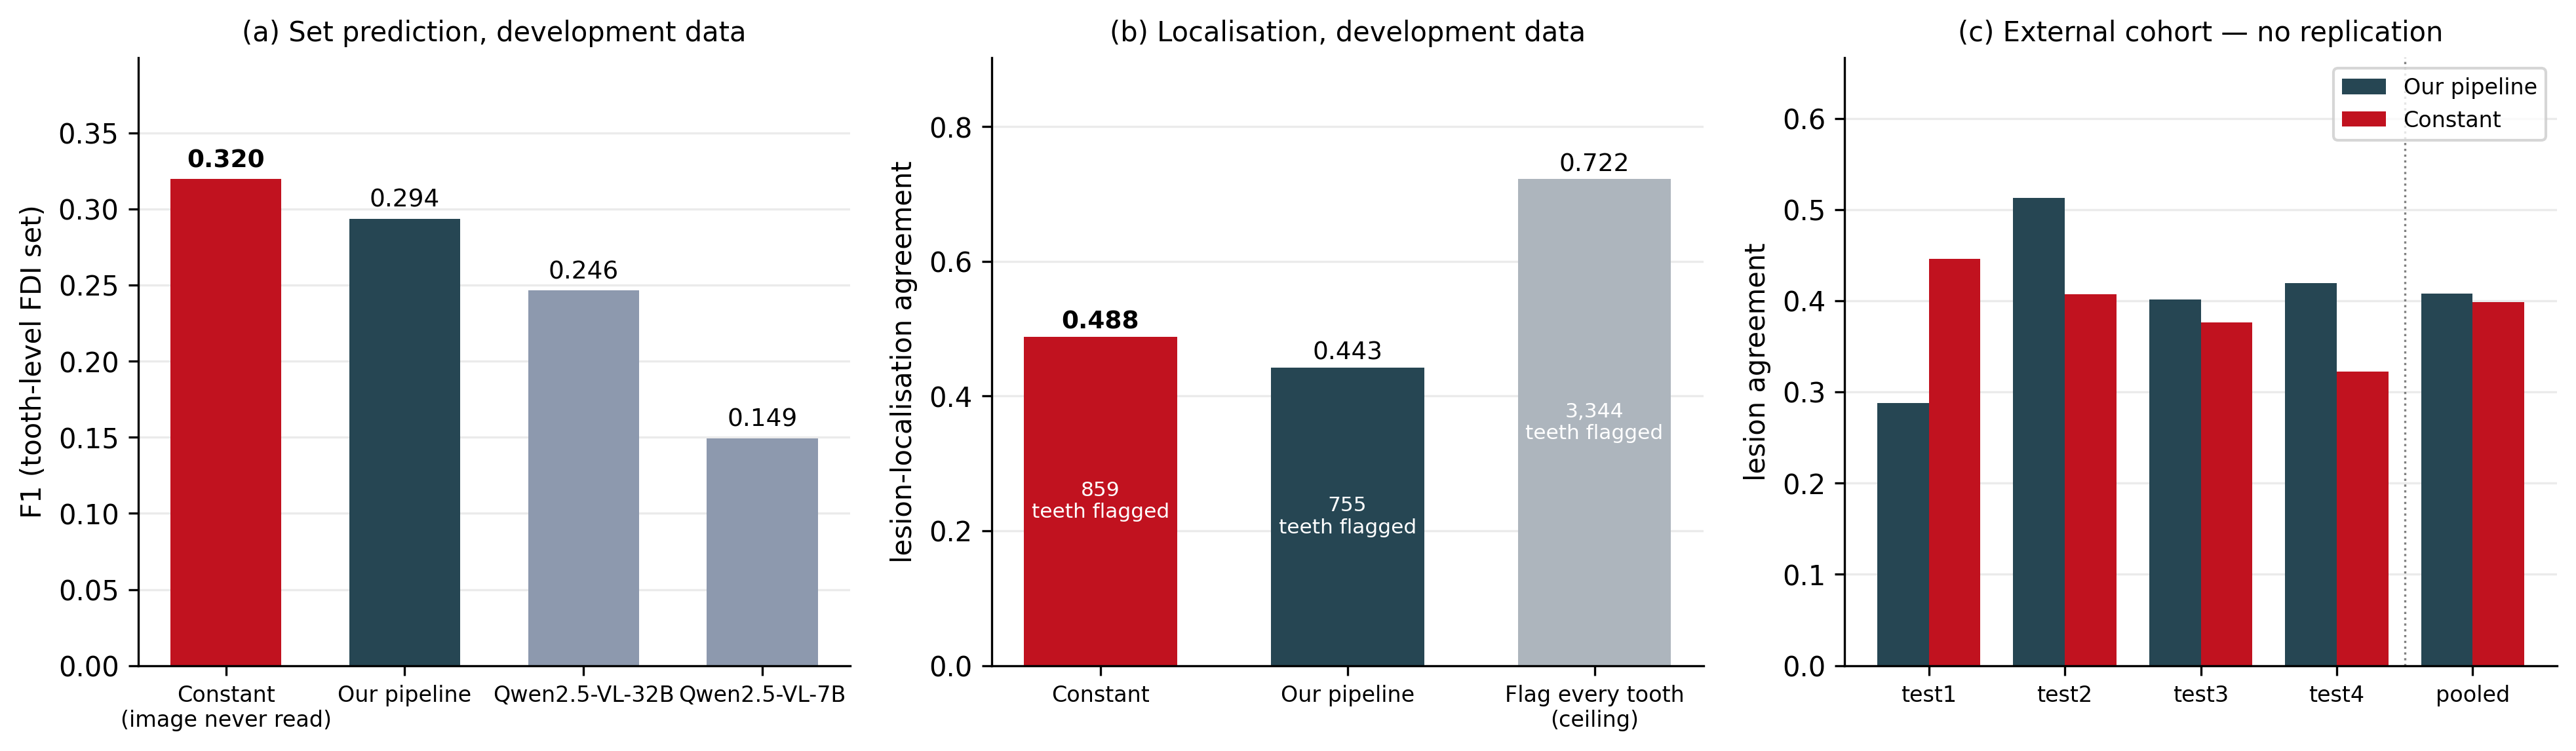
\includegraphics[width=\textwidth]{fig_baselines.png}
\caption{The constant-baseline comparison. \textbf{(a)} Tooth-level FDI-set F1 on
164 leakage-free DENTEX development images (477 annotated carious teeth). Both
vision--language models score below a constant that never reads a radiograph; the
pipeline scores above it, by an amount that depends on its caries stage.
\textbf{(b)} A second, unrelated metric on the same images (479 annotated
lesions), requiring the flagged tooth to overlap the lesion in space. Teeth
flagged is annotated inside each bar because agreement is recall-shaped, and the
flag-everything arm shows the metric's upper bound. \textbf{(c)} The external
cohort (337 images, 1{,}013 lesions, four hospitals), where the development lead
does not replicate: the difference swings 31 points between sites and vanishes
when pooled. Panels (a) and (b) are in-domain for the tooth detector and are not
comparable to (c): different cohorts and different lesion matchers
(Section~\ref{sec:protocol}). Every value is read from the saved evaluation
artefacts at render time rather than transcribed.}
\label{fig:baselines}
\end{figure*}

\subsection{The ladder on development data}

Fig.~\ref{fig:baselines} summarises the comparison; Table~\ref{tab:fdiset} gives
the set-prediction result exactly.

\begin{table}[t]
\caption{Tooth-level caries prediction. \textbf{Dataset:} 164 leakage-free
DENTEX images, in-domain for the tooth detector. \textbf{Task:} name the carious
teeth. \textbf{Metric:} FDI-set precision/recall/F1, micro-averaged.
\textbf{Unit:} tooth code; $n = 477$ annotated carious teeth. One scorer for all
arms. The pipeline is scored with each Stage-3a implementation; its parameter
counts are for the caries path.}
\label{tab:fdiset}
\centering
\footnotesize
\setlength{\tabcolsep}{3pt}
\begin{tabular}{lrrrr}
\toprule
System & Precision & Recall & F1 & Params \\
\midrule
Pipeline, lesion detector          & 0.439 & 0.574 & \textbf{0.498} & 72.99\,M \\
Pipeline, per-crop gate            & 0.237 & 0.765 & 0.362 & 58.85\,M \\
\textbf{Constant} (never reads image) & 0.218 & 0.600 & 0.320 & 0 \\
Qwen2.5-VL-32B-Instruct, 0-shot    & 0.250 & 0.243 & 0.246 & 33.45\,B \\
Qwen2.5-VL-7B-Instruct, 0-shot     & 0.248 & 0.107 & 0.149 & 8.29\,B \\
\midrule
\textit{Oracle constant (test-fitted)} & \textit{0.245} &
\textit{0.505} & \textit{0.330} & \textit{0} \\
\bottomrule
\end{tabular}
\end{table}

Read from the bottom, the ordering is inverted with respect to the information
each system receives. Both vision--language models see the radiograph and score
below a list that does not, by $+7.32$ percentage points, 95\,\% CI
$[+3.42, +11.23]$, and by $+17.04$ $[+12.66, +21.22]$. The gap between the frozen
constant and the test-set-fitted oracle is one percentage point---so almost all
of the image-blind score is available without any access to the evaluation data.

Our pipeline scores above the constant, and how far above depends on the question
its caries stage asks. With the per-crop gate it leads by $+4.27$ points, CI
$[+1.58, +7.05]$: it recovers more of the carious teeth than the constant (recall
0.765 against 0.600) at much the same precision, by naming 1{,}537 teeth where the
constant names 1{,}312. With the lesion detector it leads by $+17.80$ points
$[+13.48, +22.02]$, and does so on precision---0.439 against 0.218---while naming
fewer than half as many teeth as the constant. Section~\ref{sec:leverb} returns
to that difference. Both leads are measured on a corpus the tooth detector was
trained on (Section~\ref{sec:data}), and the question the remaining tables ask is
what is left of them once that advantage is removed.

A single metric is a single view. We therefore repeated the comparison under
lesion localisation, which demands spatial correspondence
(Table~\ref{tab:lesion}).

\begin{table}[t]
\caption{Lesion localisation. \textbf{Dataset:} the same 164 DENTEX images.
\textbf{Task:} flag a tooth overlapping each annotated lesion. \textbf{Metric:}
agreement (recall-shaped; no negative class). \textbf{Unit:} lesion; $n = 479$
annotated caries lesions. Teeth flagged is reported because agreement alone
rewards flagging more.}
\label{tab:lesion}
\centering
\small
\setlength{\tabcolsep}{4pt}
\begin{tabular}{lrrr}
\toprule
System & Agreement & Teeth flagged & Match rate \\
\midrule
Pipeline, per-crop gate   & \textbf{0.802} & 1{,}439 & 0.267 \\
\textbf{Constant}             & 0.630          & 988 & 0.306 \\
Pipeline, lesion detector & 0.595          & 603 & 0.473 \\
\textit{All teeth (ceiling)}  & \textit{0.998} & \textit{4{,}132} &
\textit{0.116} \\
\bottomrule
\end{tabular}
\end{table}

Here the per-crop pipeline leads the constant by \textbf{17.12 percentage
points}, 95\,\% CI $[+12.15, +21.89]$. Part of that lead is volume: it flags
46\,\% more teeth than the constant, at a lower match rate (0.267 against 0.306),
and this metric rewards flagging---the arm that flags every detected tooth
reaches 0.998. The lesion detector flags fewer teeth than either, at the highest
match rate of the three (0.473), and its agreement is not separable from the
constant's: $-3.55$ points, CI $[-10.11, +2.64]$.

On development data, then, the pipeline is above the image-blind constant under
one metric, and above or level with it under the other depending on its caries
stage. Neither statement is yet evidence of perception, because the front end
that places every flagged tooth---the constant's included---was trained on this
corpus.

\subsection{The ladder on external data}

We then ran the same comparison on four hospitals the system had never seen
(Table~\ref{tab:external}). The rows score the pipeline with its per-crop gate,
the stage this comparison was designed around; Section~\ref{sec:leverb} gives the
lesion detector on the same images.

\begin{table}[t]
\caption{External validation. \textbf{Dataset:} four hospitals, 337 images.
\textbf{Task:} flag a tooth containing each lesion centroid. \textbf{Metric:}
lesion agreement by centroid containment---a different matcher from
Table~\ref{tab:lesion}, for the reason given in Section~\ref{sec:protocol}.
\textbf{Unit:} lesion; $n = 1{,}013$. $\Delta$ is constant minus pipeline.}
\label{tab:external}
\centering
\small
\begin{tabular}{llrrrr}
\toprule
Hospital & Centre & Lesions & Pipeline & Constant & $\Delta$ (pp) \\
\midrule
test1 & cross      & 316 & 0.519 & \textbf{0.709} & $+19.0$ \\
test2 & same\,$^{a}$ & 349 & \textbf{0.702} & 0.579 & $-12.3$ \\
test3 & cross      & 162 & 0.512 & 0.494 & $-1.9$ \\
test4 & cross      & 186 & 0.624 & 0.500 & $-12.4$ \\
\midrule
\textbf{Pooled} & --- & 1{,}013 & 0.600 & 0.591 & $-0.89$ \\
\bottomrule
\end{tabular}

\vspace{2pt}
\raggedright\footnotesize
$^{a}$ Same centre as the \emph{source cohort's own} training portion. No
Ningxia data was used to train or tune our system; all four splits are equally
external to us (Section~\ref{sec:data}).
\end{table}

\textbf{The development-set lead does not replicate.} Pooled, the difference is
$-0.89$ percentage points with 95\,\% CI $[-5.57, +3.86]$: the two systems are
statistically indistinguishable, with the pipeline nominally ahead by an amount
the interval cannot separate from zero.

The per-site spread is the more useful observation. The difference swings from
$+19.0$ points at test1 to $-12.3$ at test2, both intervals excluding zero---a
31-point range across hospitals of a single cohort---and the pooled figure conceals
this entirely.
test1 is the constant's best site by a wide margin and one of the pipeline's two
worst. We do not have an explanation for that, and we report it unexplained
rather than omit it.

\textbf{A second external cohort makes the point sharper still.} We repeated the
identical comparison, with the same matcher and the same frozen system, on the
published CariesXrays benchmark~\cite{chen2024cariesxrays}---1{,}200 images
carrying 2{,}815 lesions, more than the development and Ningxia
cohorts combined (Table~\ref{tab:cohorts}). There the constant does not merely
tie: it wins by \textbf{22.42 percentage points}, 95\,\% CI $[+20.18, +24.62]$.

\begin{table}[t]
\caption{The same comparison across three cohorts: the pipeline with its per-crop
gate against the constant. \textbf{Metric:} lesion agreement by centroid
containment for the two external rows; the development row uses the matcher of
Table~\ref{tab:lesion} and is not comparable in absolute value. \textbf{Unit:}
lesion. $\Delta$ is constant minus pipeline; intervals are paired cluster
bootstraps over images.}
\label{tab:cohorts}
\centering
\footnotesize
\setlength{\tabcolsep}{3pt}
\begin{tabular}{lrrrl}
\toprule
Cohort & Lesions & Pipeline & Constant & $\Delta$ (pp), 95\,\% CI \\
\midrule
DENTEX (dev.) & 479   & \textbf{0.802} & 0.630 & $-17.12\ [-21.89, -12.15]$ \\
Ningxia (4 hosp.) & 1{,}013 & 0.600 & 0.591 & $-0.89\ [-5.57, +3.86]$ \\
CariesXrays & 2{,}815 & 0.379 & \textbf{0.604} & $\mathbf{+22.42\ [+20.18, +24.62]}$ \\
\bottomrule
\end{tabular}
\end{table}

Two observations follow, and the second is the one that matters. First,
\textbf{volume explains part of one result and none of the other}. On the
development set the pipeline's lead came with 46\,\% more flagged teeth at a
lower match rate. On CariesXrays the roles reverse and the explanation fails: the
constant flags 46\,\% more teeth \emph{and} attains the higher hit rate (0.200
against 0.188). It is ahead on both axes.

Second, \textbf{the size of the gap is a property of the cohort, not of the
systems}. The constant's own agreement on CariesXrays, 0.604, is the share of
that cohort's lesions lying on the eight teeth it names. Where caries
concentrates in the molars to that degree, an anatomical prior is close to
optimal by construction.

Taken together the three cohorts place the same pipeline 17 points above the
constant, level with it, and 22 points below it, depending only on which
cohort is scored---and the one cohort on which it leads is the one its tooth
detector was trained on. The swing across a single cohort's four sites is 31
points; the swing across cohorts is 40. \textbf{A tooth-level agreement figure
reported on one cohort therefore carries almost no information about a system's
perceptual ability}, and a favourable one on development data carries least of
all.

\subsection{Changing the task, not the architecture}
\label{sec:leverb}

The external tables above score the per-crop gate of Section~\ref{sec:lesiondet}.
Five attempts to repair that gate directly---contrast equalisation, crop
expansion, position-balanced sampling, a retrained gate, and threshold
tuning---all returned intervals spanning zero. We therefore changed the question
rather than the model, and replaced the gate with the whole-image lesion
detector. The decision rule was registered and committed before any arm was
trained: to be adopted, the detector had to beat both the constant and the gate,
on at least two of three cohorts, at no more than $1.5\times$ their rate of
flagging teeth.

\textbf{The rule was met on two cohorts of three.} It was applied to the pipeline
as it then stood, with a tooth detector trained on Tufts alone: the lesion
detector led the constant by $+12.2$ points $[+10.1, +14.3]$ on CariesXrays and by
$+10.2$ $[+6.3, +14.0]$ on Ningxia, and tied it on DENTEX at $-3.3$
$[-8.4, +1.3]$. The bar was not moved after the numbers were seen.
Table~\ref{tab:leverb} reports the same three arms under the current tooth
detector. It is a description, not a second verdict, and the pattern is the one
the rule was met on: ahead on both external cohorts, level on DENTEX. We report
DENTEX as a tie everywhere it appears.

\begin{table}[t]
\caption{Stage 3a reformulated as lesion detection, under the current tooth
detector. \textbf{Metric:} tooth-level lesion agreement, matched exactly as in
Table~\ref{tab:cohorts}. \textbf{Unit:} lesion. Within a cohort all three arms
score the same images, and each row is the same cohort as in
Table~\ref{tab:cohorts}; intervals are paired cluster bootstraps over images
(10{,}000 resamples). Lesion counts are 479, 2{,}815 and 1{,}013 by row.}
\label{tab:leverb}
\centering
\footnotesize
\setlength{\tabcolsep}{3pt}
\begin{tabular}{lrrrl}
\toprule
Cohort & Gate & Const. & Lesion & $\Delta$ vs const. (pp) \\
\midrule
DENTEX$^{d}$      & 0.802 & 0.630 & 0.595 & $-3.55\ [-10.11, +2.64]$ \\
CariesXrays$^{d}$ & 0.379 & 0.604 & \textbf{0.757} & $\mathbf{+15.38\ [+12.96, +17.73]}$ \\
Ningxia$^{e}$     & 0.600 & 0.591 & \textbf{0.684} & $\mathbf{+9.28\ [+4.72, +13.73]}$ \\
\bottomrule
\end{tabular}

\vspace{2pt}
\raggedright\footnotesize
$^{d}$ Development data for the lesion detector: a corpus it trained on, scored on
images it did not train on; for CariesXrays those are its validation split, on which
its checkpoint was chosen. $^{e}$ External: never trained on or tuned against, but one
of the three cohorts that decided this detector's adoption.
\end{table}

Four things about this result are worth more than the margin itself.

\textbf{It is not a volume effect.} The objection we raised against the constant
applies here in reverse, so we apply it. The detector flags \emph{fewer} teeth than
either comparator on every cohort---2.16 per image against the constant's 7.05 on
CariesXrays, 4.35 against 7.15 on Ningxia---so it is not buying agreement by
flagging more.

\textbf{It holds, pooled, on the one cohort that is genuinely external.} The
Ningxia row of Table~\ref{tab:leverb} scores the same 337 images, the same
1{,}013 lesions and the same constant as the Ningxia row of
Table~\ref{tab:cohorts}. On that fixed comparison the gate was $0.89$ points ahead
of the constant and could not be separated from it; the detector is $9.28$ points
ahead with an interval excluding zero. Per hospital it is separated from the
constant at test2, test3 and test4 ($+16.91$ $[+9.17, +24.62]$, $+11.73$
$[+1.07, +21.34]$ and $+13.98$ $[+2.34, +24.34]$) and not at test1 ($-3.16$
$[-10.56, +3.97]$), the hospital where the constant is strongest. It was the first
arm in this work to beat the constant on data it had never seen. Because Ningxia was
one of the three cohorts that decided the detector's adoption, this lead is
conditioned on that choice: its sign is robust, its size optimistic. Under the
previous tooth detector the same two comparisons were $+0.79$ and $+10.07$ points;
only on DENTEX did a sign change with the detector.

\textbf{The training mixture, not the detector, is what transfers.} A second arm
trained on CariesXrays alone was scored beside the pooled one when the rule was
applied. It reached $0.694\ [0.674, 0.714]$ on CariesXrays, a shade above the
pooled arm's $0.684$ on that pipeline, and then collapsed to
$0.086\ [0.055, 0.119]$ on DENTEX and $0.240\ [0.209, 0.272]$ on Ningxia---far
below even the constant. Judged on its own corpus the two arms look like the same
model, and the single-corpus one looks slightly better. Judged anywhere else, it
does not work. We could not have told them apart without the external cohort,
which is the argument of this paper applied to our own result.

\textbf{One comparison went against it when the tooth detector changed}, and we
print it for that reason. On DENTEX lesion agreement the per-crop gate now scores
above the lesion detector, 0.802 against 0.595 ($-20.67$ points, CI
$[-26.39, -15.06]$), where the two had been level. The gate reaches that figure by
flagging 1{,}439 teeth to the detector's 603; on FDI-set F1, which charges for
false positives, the order is reversed (0.362 against 0.498). Which of the two a
reader should prefer depends on what a wrongly flagged tooth costs, and we do not
settle that here.

\subsection{What the constant cannot do}
\label{sec:numbering}

A constant answers a set-membership question. It cannot perform tasks whose
output is not a fixed list, and the pipeline's results on those tasks are
correspondingly meaningful.

\begin{figure*}[t]
\centering
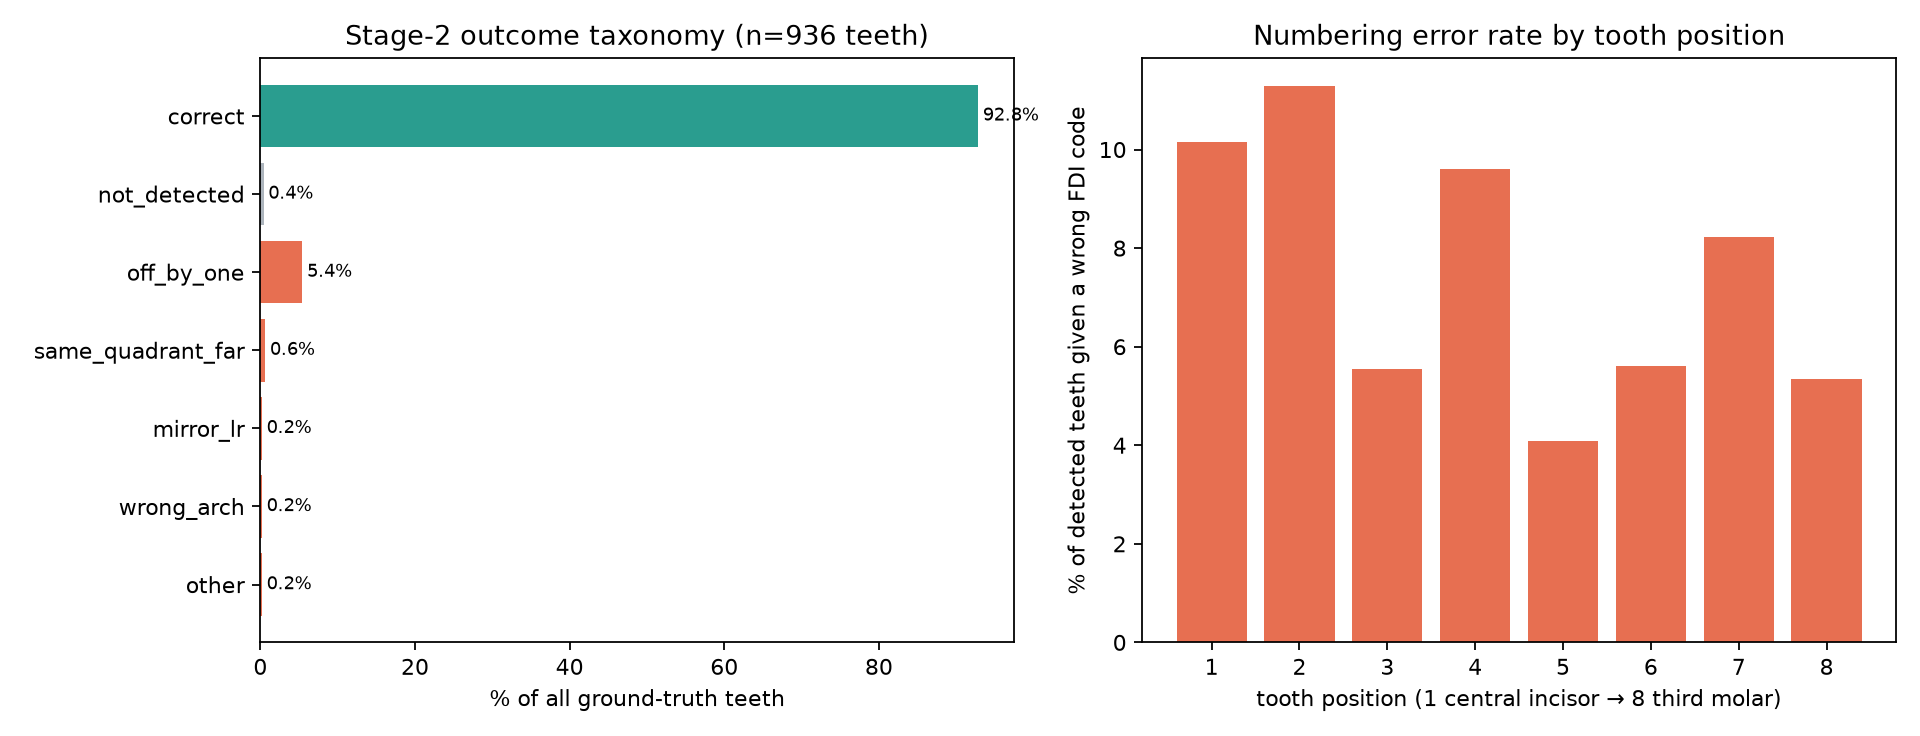
\includegraphics[width=\textwidth]{fig_stage2.png}
\caption{Where the numbering stage loses teeth, over 936 ground-truth teeth in
164 DENTEX images, in-domain for the tooth detector. Almost every tooth is
proposed and numbered correctly; among the codes that are wrong, most are
off-by-one within the correct quadrant.}
\label{fig:stage2}
\end{figure*}

\textbf{Tooth numbering.} End-to-end FDI-exact accuracy on DENTEX is 92.8\,\%
($869/936$ teeth), 95\,\% CI $[90.6, 94.9]$. It is an \textbf{in-domain} figure
and we report it as one: the 164 images are held out, but the tooth detector was
trained on other images of the same corpus. Four of the 936 teeth (0.4\,\%) are
never detected, and of the 932 that Stage 1 does find, Stage 2 numbers
\textbf{93.2\,\%} correctly. It is this second figure that compares to the
pre-cropped accuracies in Section~II.

On the held-out Tufts test split---3{,}760 teeth, every tooth in the mouth rather
than only those carrying a finding---the same pipeline reaches \textbf{63.5\,\%}
end to end, CI $[59.3, 67.5]$: 89.3\,\% of teeth are detected and 71.1\,\% of
those numbered correctly. Tufts too is a corpus the detector was trained on. On
UFBA-425, which neither the detector nor the numbering head trained on, the pipeline
reaches 44.5\,\% end to end, CI $[42.39, 46.62]$ (recall 66.6\,\%), on the square
export as distributed, and 77.2\,\% $[75.19, 79.14]$ (recall 95.6\,\%) with each
image widened to a panoramic shape, an aspect ratio we have not verified for these
files. That is one corpus and a single pass; on it the adopted detector leads the
one it replaced by $+23.86$ points $[+21.96, +25.77]$.

Residual errors on DENTEX are mostly near misses: of 63 incorrect codes, 51
(81.0\,\%) name an adjacent tooth within the correct quadrant, and only 6 of 932
detected teeth (0.6\,\%) receive an error at the quadrant level---naming a tooth
in the wrong corner of the mouth. A constant cannot attempt this task at all.

\begin{figure}[t]
\centering
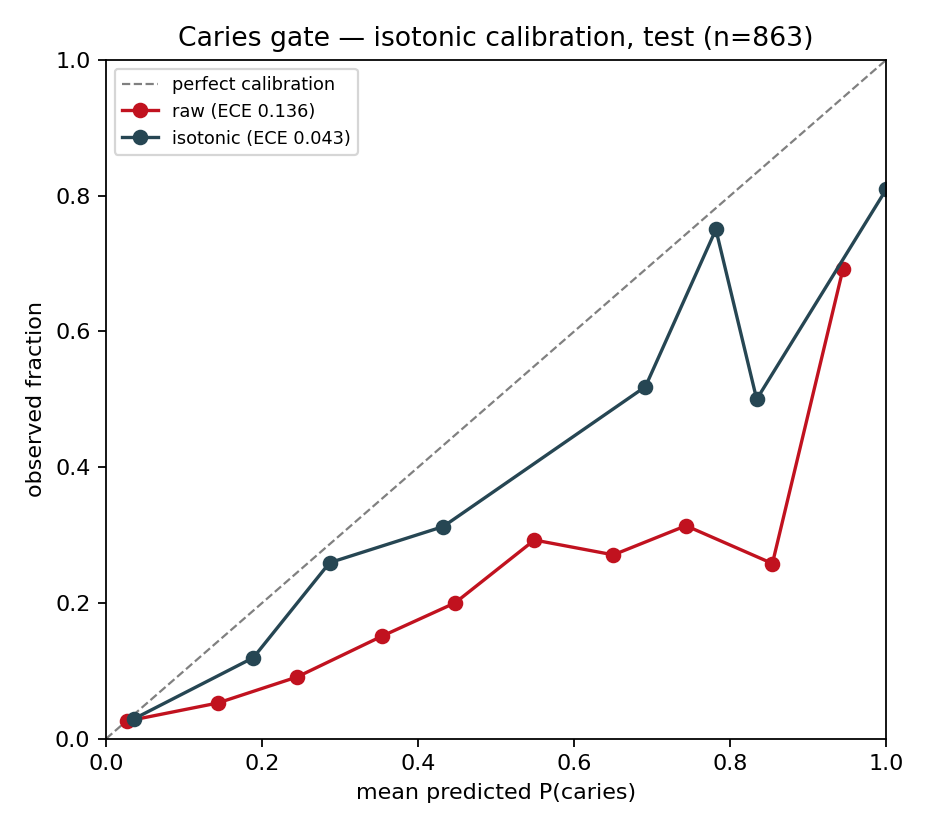
\includegraphics[width=\columnwidth]{fig_calibration.png}
\caption{Reliability of the caries \emph{gate} --- the retained Stage-3a variant,
not the adopted lesion detector --- before and after isotonic regression, on 863
held-out test crops. The uncorrected model is systematically overconfident: at a
stated confidence of 0.85 the observed frequency of caries is 0.26.}
\label{fig:calib}
\end{figure}

\textbf{Calibration.} \emph{Calibration} asks whether a model's confidence
behaves like a probability: of the teeth it calls carious with 80\,\%
confidence, are 80\,\% actually carious? \textbf{Expected calibration error}
(ECE) is the average gap between stated confidence and observed frequency across
confidence bins; 0 is perfect.

Everything in this subsection that concerns caries was measured on the
\textbf{per-crop gate}, which since Section~\ref{sec:leverb} is the retained
Stage-3a variant rather than the default. We state the consequence rather than
leave it implied: the adopted lesion detector emits a detection score, not a
posterior over a tooth, so it has no reliability diagram, no calibrator and no
abstention curve of its own, and we do not claim one for it
(Section~\ref{sec:limits}). The numbering results below are unaffected---Stage~2
did not change---and they are what the two capabilities look like in the system
as it ships today.

The caries gate's confidences are not probabilities. Its ECE is \textbf{0.136}
and every reliability bin lies below the diagonal---it is systematically
overconfident. Temperature scaling~\cite{guo2017calibration}, the standard first
remedy, made calibration \emph{worse} (0.152), indicating the miscalibration is
structural rather than a single scale factor. Isotonic
regression~\cite{zadrozny2002isotonic} reduced ECE to \textbf{0.043}.

That improvement is not free, and we report its cost. Isotonic regression is only
weakly monotonic: on this model it collapses the test scores to 46 distinct
values and average precision falls from \textbf{0.550 to 0.500}. Applied at the
decision threshold it would also change \textbf{155 of 863 verdicts (18\,\%)}. We
therefore apply it to the \emph{reported confidence only}, leaving each verdict as
the raw \texttt{argmax}, so that every published caries number in this paper is
the one that was measured. This is a deployment choice with a stated price, not a
property of the method---and it is the opposite of temperature scaling, which
cannot change a verdict but did not fix the calibration.

One number should accompany all of this: the gate's average precision is
\textbf{0.550} $[0.445, 0.660]$ against a prevalence of 0.147, i.e. 3.7$\times$
chance. What fails is calibration and the operating point, not the model's
ability to rank teeth.

\begin{figure}[t]
\centering
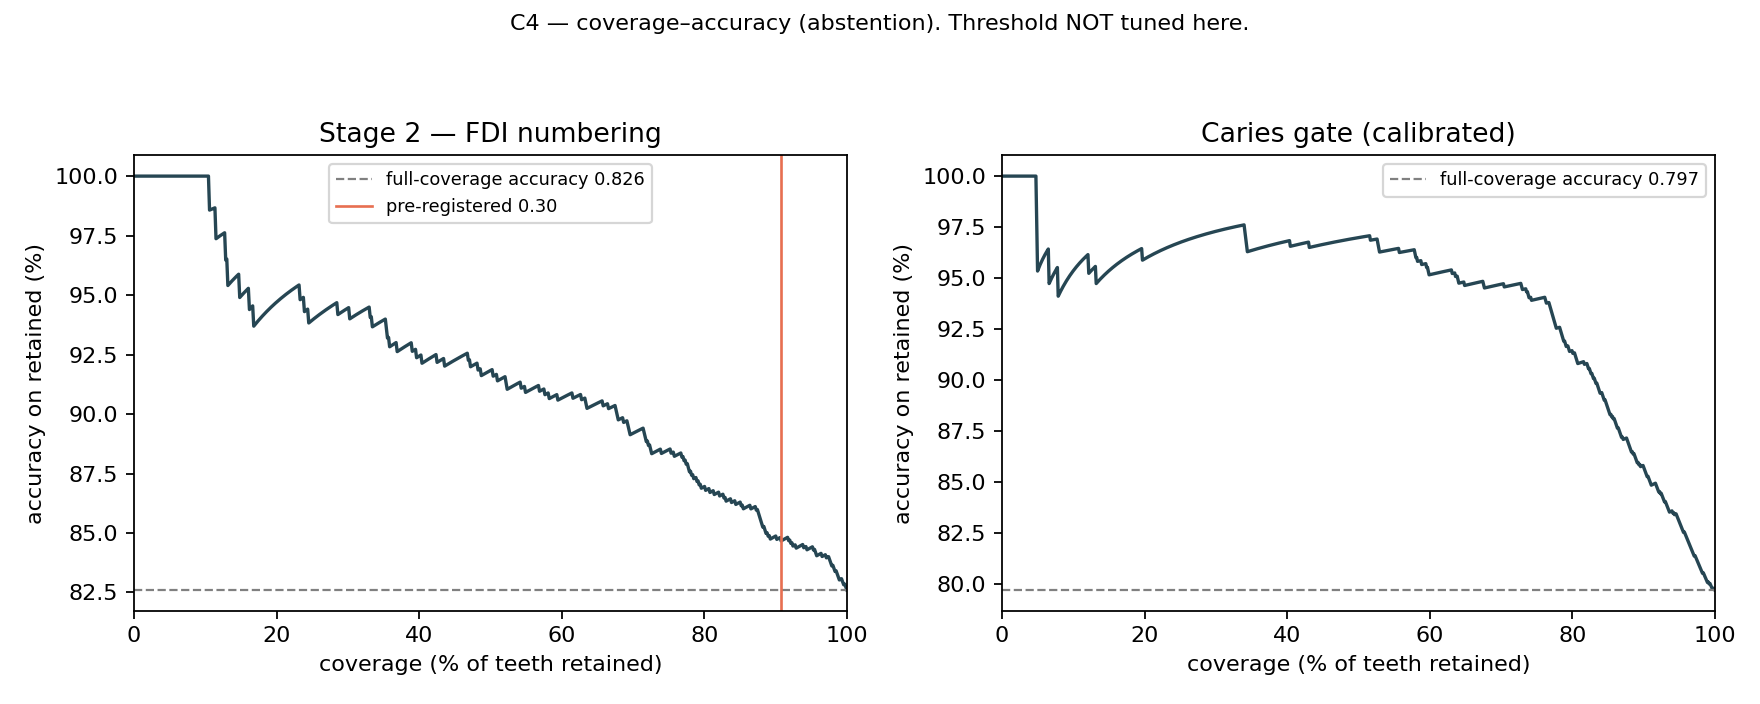
\includegraphics[width=\columnwidth]{fig_coverage.png}
\caption{Coverage--accuracy for tooth numbering (left) and the caries \emph{gate}
(right); the caries panel is the retained Stage-3a variant, not the adopted lesion
detector. Accuracy on retained predictions rises as the least-confident cases are
declined. The vertical line marks the pre-registered threshold of 0.30, located
on the curve rather than tuned against it.}
\label{fig:coverage}
\end{figure}

\textbf{Selective prediction.} A system may be allowed to \emph{decline}---to
answer ``I am not confident enough on this tooth'' instead of guessing.
\emph{Coverage} is the fraction of cases it still answers; accuracy is then
measured on those alone. This is only useful if the model's confidence actually
identifies its own errors.

Declining the least-confident quarter of cases raises numbering accuracy from
0.932 to \textbf{0.980} ($+4.76$ pp, CI $[+3.29, +6.54]$, 164 image clusters) and
caries-gate accuracy from 0.797 to \textbf{0.940} ($+14.25$ pp, CI
$[+11.32, +16.63]$, 34 image clusters). Under the shuffle control both gains
collapse to $-0.06$ and $+0.00$ percentage points, establishing that the
improvement comes from the confidence ranking and not from discarding items.

The pre-registered threshold of 0.30 lands at 96.1\,\% coverage and 0.941
accuracy. It was chosen before these data were seen, and on this corpus it
declines little: at 90\,\% coverage the empirical accuracy is 0.955.

One caveat must accompany any coverage figure here: coverage is measured over
\emph{detected} teeth. Retaining 75\,\% of detections corresponds to 75\,\% of
99.6\,\%, or \textbf{74.7\,\% of the teeth actually present in the mouth}, on a
corpus where nearly every tooth is found. Where the detector finds fewer, the
same sentence has to be recomputed.

\subsection{Vision--language model behaviour}

Few-shot prompting, with exemplars drawn strictly from leakage-excluded images,
degrades the smaller model monotonically: F1 falls from 0.149 zero-shot to 0.066
at two shots and 0.034 at four. The mechanism is abstention rather than
error---empty answers rise from 56 of 164 images to 123 of 164---so exact-set
match simultaneously \emph{rises}, because 16 images contain no caries and an
empty answer scores an exact match on each. Reported alone, that column would be
true and thoroughly misleading.

The content-free controls are more direct, and the two models behave differently
enough that they must be reported separately.

\begin{itemize}
  \item \textbf{Qwen2.5-VL-7B-Instruct} answers \texttt{26,36} to a blank grey
        image and \texttt{26,36} to random noise---identical to its answer for a
        real radiograph.
  \item \textbf{Qwen2.5-VL-32B-Instruct} answers \texttt{NONE} to the blank
        image, which is correct behaviour. Shown random noise, it answers
        \texttt{16, 17, 26, 27, 36, 37, 46, 47}---\emph{exactly} the eight-molar
        set our greedy search recovered from the data, and identical to its
        answer for a real radiograph.
\end{itemize}

The larger model therefore detects the absence of an image but not the absence of
anatomy, and what it emits in that condition is the population prior itself.
Whatever these outputs measure on a noise input, it is not perception of the
image in front of them. We claim this for these two models under this prompt, and
no further.

The efficiency comparison survives all of the above: 33.45\,B parameters and
70.1\,GB of accelerator memory are outscored by 72.99\,M parameters running on a
CPU---a factor of roughly 460 in parameter count, in the wrong direction for the
larger model.

\subsection{Stage 4: an abnormality flag, measured held out}
\label{sec:stage4}

\begin{figure}[t]
\centering
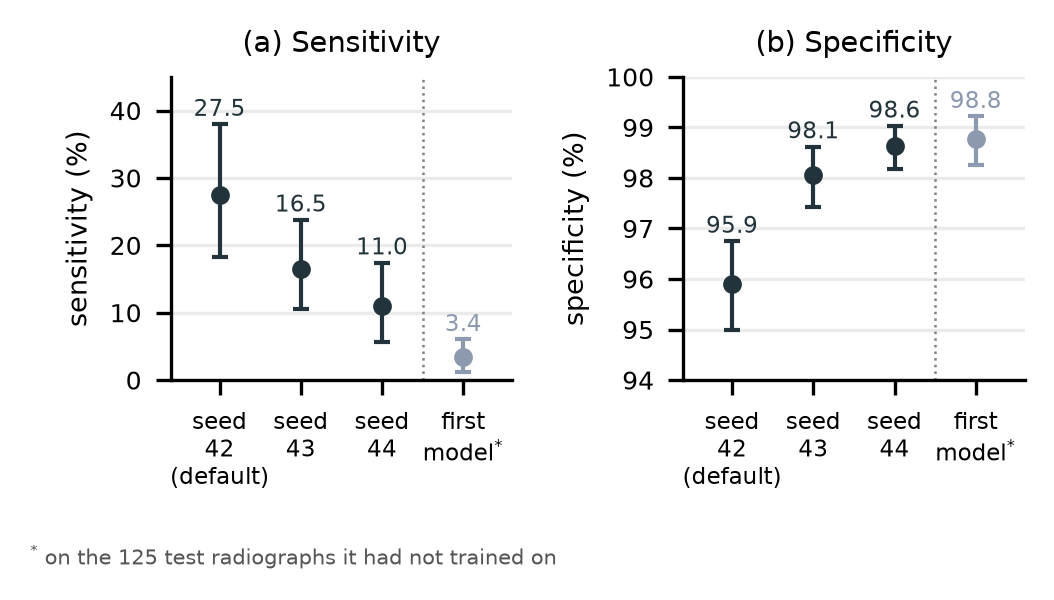
\includegraphics[width=\columnwidth]{fig_stage4a.png}
\caption{Stage 4 on the held-out Tufts test split (143 radiographs, 3{,}892
teeth, 182 carrying its label): three training runs of one recipe, each with a
95\,\% interval from a bootstrap over radiographs, beside the first model on the
125 of those radiographs it had not trained on. The intervals cover the sampling
of radiographs, not the training run; the spread between runs is the larger
uncertainty. The axis in (b) is truncated.}
\label{fig:stage4}
\end{figure}

Stage 4 was built to flag periodontal bone loss, and it is not a periodontal
detector. It is a ResNet18 that flags teeth whose crop overlaps an
expert-marked abnormality on Tufts---described by that expert as apical lesions,
sclerosis and cysts---so we name it for that label. The model first shipped
reported 0.923 macro-F1 and 83\,\% sensitivity from a crop-level split in which
every validation radiograph also supplied training crops; on the 125 test
radiographs it had not trained on, it found \textbf{3.4\,\%} of such teeth (6 of
175). Retrained with the split made by radiograph, under a protocol written down
before training, three runs of one recipe found \textbf{27.5\,\%, 16.5\,\% and
11.0\,\%} of such teeth on 143 test radiographs (50, 30 and 20 of 182; 18.3\,\%
pooled), at 95.9--98.6\,\% specificity, with about seven flags in ten false
(precision 24.8--29.4\,\%; Fig.~\ref{fig:stage4}). The runs rank teeth alike
(ROC area 0.68--0.69) and differ in operating point; the ranking is separated from
a tooth-position prior on average precision and not on ROC area. The run whose
seed was fixed in advance, the 27.5\,\% one, is the pipeline default; that choice
was made with the test result in view, and we do not call it pre-registered.

These figures were scored on annotated tooth boxes, not on the pipeline's own
detections, and the flag has no external figure: on the 164 DENTEX images, which
carry no such label, it fires on 6.1\,\% of detected teeth (274 of 4{,}512), a
rate and not a sensitivity. The three runs share one pre-computed set of jittered
training crops, so their spread understates training variance, and every interval
covers the sampling of radiographs only. One of the 143 test radiographs is a
re-rendered copy of a training radiograph; it holds no positive tooth. A second
ResNet18, meant to grade the flagged teeth, was trained on bands of crop contrast,
a stand-in for an overlap measurement its training data lacked; it is present in
the released code, withheld from the report by default, and not evaluated. We
make no periodontal claim.

%% =====================================================================
\section{Discussion}
%% =====================================================================

\subsection{Main finding}
On our development data an image-blind constant outscored two vision--language
models, and a purpose-built six-stage pipeline cleared it---by four points with
one caries stage and eighteen with another---under a tooth detector trained on
that corpus. On four external hospitals the pipeline with its per-crop stage and
the constant could not be separated at all, and on a second external benchmark
the constant led by 22 points. The finding is therefore not that the constant
wins---it does not, reliably---nor that the pipeline does, but that \textbf{these
metrics cannot tell the two apart outside the data a system was built on}, which
is a stronger and more troubling result than either outcome alone.

That conclusion is about a task, and it survives being acted on. Reformulating
Stage 3a from per-tooth classification to lesion detection---the same backbone
family, no supervision beyond boxes the corpora already carried---moved the
external comparison from a tie to a $9.28$-point lead over the constant, on the
same 337 images and the same metric (Section~\ref{sec:leverb}). What changed was
the question the model was asked, not how well it was asked. We read the two
results as one finding rather than two: a tooth-level agreement figure is
uninformative about perception, and the way past that is to score something the
prior cannot produce---not to build a better classifier of the same thing.

\subsection{Why the floor is high, and why that is not a criticism of any model}
Caries in these cohorts is anatomically concentrated: molars carry most of the
disease. A tooth-level decision is a set-membership question over a fixed
vocabulary of 32 codes, and set membership inherits that concentration directly.
A fixed answer naming the eight first and second molars is not a degenerate
output---it is a compact statement of dental epidemiology, and it is right for
the same reason a clinician's prior is right.

The consequence is that the headroom above such an answer is small, and small
\emph{independently of model quality}. No amount of architectural work raises a
ceiling imposed by the pairing of task and metric. A system distinguishes itself
here only by being right about \emph{this patient} in a way the population prior
is not, and tooth-level set membership is a poor instrument for detecting that
difference.

We treated that as a claim to be tested rather than a rhetorical flourish, and it
held in both directions. Five separate repairs to the classifier returned intervals
spanning zero; the ceiling moved only once the pairing itself did
(Section~\ref{sec:leverb}).

The floor also moves with the front end, which is the detail we did not
anticipate. Changing only the tooth detector raised the per-crop pipeline's
lesion agreement on every cohort---and raised the constant's with it, by $+13.99$,
$+4.12$ and $+19.25$ points on the three cohorts, because the constant's eight
codes are placed on the image by the pipeline's own boxes and numbering. An
improvement of that kind is real and worth having. It is not evidence that the
caries stage reads lesions any better, and only the comparison against the
constant, which received the same improvement, can tell the two apart.

\subsection{Why the external disagreement changes the interpretation}
We expected the external cohort to confirm the development result. It did not.
Pooled, the two systems are indistinguishable; per site, the difference swings
through 31 points.

Two readings remain open and we cannot separate them with the data we have.
Either the development lead is partly a property of DENTEX---of its particular
caries distribution, or of the tooth detector having trained on it---or the
external metric, which must use centroid containment for the geometric reason
given in Section~\ref{sec:protocol}, has different sensitivity to the same
underlying effect. We report the ambiguity rather than resolve it by assertion.

What the disagreement does establish is firmer than what it leaves open: at this
variance, \emph{a single external number carries very little information}. Our
own pooled 0.600 is, in isolation, as uninterpretable as any other pooled figure
in this literature, including the ones we cite. One hospital in our cohort would
have supported the claim that the constant wins decisively; another would have
supported the opposite. Reporting either alone would have been defensible,
publishable, and wrong.

\subsection{What the system can still demonstrate}
\label{sec:demonstrate}
A constant cannot name a tooth, cannot express a calibrated confidence, cannot
decline informatively, and has no behaviour under domain shift to measure. We
propose these as the axes on which OPG systems should be compared, with our own
figures as an illustration of what reporting them looks like:

\begin{enumerate}
  \item \textbf{Identification}---can it say \emph{which} tooth? Here 93.2\,\% of
        detected teeth on one in-domain corpus and 71.1\,\% on another, with
        detection recall of 99.6\,\% and 89.3\,\% stated alongside.
  \item \textbf{Calibration}---do its confidences behave like probabilities? For
        numbering, yes; for caries, ECE $0.136 \rightarrow 0.043$ \emph{on the
        gate variant}, with the failed temperature-scaling attempt reported
        because it diagnoses the miscalibration as structural, and with the
        0.550\,$\rightarrow$\,0.500 average-precision cost stated.
  \item \textbf{Selective prediction}---does declining improve accuracy, and does
        the gain survive a shuffle control? $+4.76$ pp for numbering and
        $+14.25$ pp for the caries gate, and yes to the control in both cases.
  \item \textbf{Domain shift}---measured on held-out institutions and reported per
        site, including when the answer is that a branch does not transfer.
\end{enumerate}

A constant scores nothing on any of these. That asymmetry, rather than a caries
F1, is what the system has to show. We hold ourselves to it: on axes 2 and 3 the
caries branch as it now ships has no result, because the stage those numbers
describe is no longer the default one (Section~\ref{sec:limits}).

\subsection{Anticipated objections}
\textbf{``Your pipeline is simply weak.''} Possibly, but that does not explain
the result. Two general-purpose models at 8.29\,B and 33.45\,B parameters were
scored by the identical scorer and placed \emph{below} the constant, and our
pipeline, which clears it on development data, could not be separated from it at
four hospitals it had never seen. An explanation resting on our system's quality
would have to account for three systems of very different design failing to
separate from the same prior once the home advantage is removed.

\textbf{``The constant was fitted, so it is not uninformed.''} It is fitted---on
78 held-out images, byte-disjoint from every scored image---and then frozen. What
it learns is a population statistic: which teeth tend to be carious, not anything
about the radiograph in front of it. That is exactly the quantity a diagnostic
claim must exceed. Its score drops from 0.392 on the fitting images to 0.320 on
the scored ones, in the direction an honest held-out fit should.

\textbf{``The metrics were poorly chosen.''} The first is the metric this
literature predominantly reports; we did not select it to make a point. The
second we introduced specifically to escape the first, and outside the
development corpus it gave the same answer. We also report the degenerate
flag-everything arm, which reaches 0.998 agreement, so the reader can judge the
metric's headroom directly.

\textbf{``A molar-prior system would still be clinically useful.''} It might well
be, and we do not dispute it. But a tool that encodes epidemiology is a different
object from a tool that reads a radiograph, and only the second can find the
lesion the prior does not expect. That distinction is invisible to the metric and
central to the clinic.

\subsection{What we propose should be reported}
\textbf{An image-blind baseline row.} One line of code, no compute, alongside any
tooth-level caries metric on this class of data. Without it a mid-range number
cannot be interpreted---the five rows of Table~\ref{tab:fdiset} span 0.149 to
0.498, and the one that reads no image sits in the middle of them.

\textbf{Per-institution results.} Pooled external figures conceal exactly the
variation that external validation exists to expose.

\textbf{Metrics with demonstrated headroom.} If a degenerate arm reaches most of
the achievable range, the metric cannot support a perception claim regardless of
what a system scores on it.

None of this invalidates prior work. It narrows one specific inference: the claim
\emph{this system perceives caries} is not established by a tooth-level number
alone.

\subsection{Clinical interpretation}
This study does not establish clinical usefulness, and nothing here should be
read as a claim about patient outcomes. We did not compare any system against a
dentist, did not evaluate prospectively, and did not measure whether a flagged
tooth changes what a clinician does. What the study does support is a narrower
statement about how such systems should be assessed before they reach a clinic:
that a tooth-level agreement score, reported without a floor and without external
per-site results, is not sufficient evidence that a screening aid is reading the
image it is shown.

\subsection{On reporting results that do not favour the authors}
Three findings here are unfavourable to our own system: an external comparison
in which it cannot be told from a constant, a fourth stage whose first score
came from a leaky split and whose held-out recall is low, and a tooth detector adopted over a registered guard it failed. We
report all three. A screening tool
that fails silently is more dangerous than one that fails visibly, and the
alternative---selecting whichever metric flatters the system---is precisely the
practice this paper argues against. We would have no standing to recommend
image-blind baselines to others while declining to survive one ourselves.

%% =====================================================================
\section{Limitations}
\label{sec:limits}
%% =====================================================================

Each item states what it prevents us from concluding.

\begin{enumerate}
  \item \textbf{The adopted caries stage has no calibrated confidence and no
        abstention curve.} The calibration and selective-prediction results of
        Section~\ref{sec:numbering} were measured on the per-crop gate, which
        Section~\ref{sec:leverb} demoted to a retained variant. The lesion
        detector that replaced it emits a detection score, and we have neither
        fitted a calibrator for it nor re-derived a coverage--accuracy curve
        against it; the pre-registered 0.30 threshold was located on the gate's
        curve and does not transfer to a quantity with a different meaning. So
        for caries, the system as it ships today demonstrates identification and
        domain-shift behaviour but neither of the middle two axes of
        Section~\ref{sec:demonstrate}. Numbering demonstrates all four. We regard
        closing this as the first piece of follow-up work, and it needs its own
        pre-registration rather than a threshold chosen once the curve is
        visible.
  \item \textbf{No clinician comparison.} We do not know how any system here
        compares against a dentist on these images. We therefore cannot claim
        clinical utility, non-inferiority, or that the constant would mislead a
        clinician less than the pipeline. This is the single largest gap.
  \item \textbf{The caries cohorts disagree in direction.} The pipeline with its
        per-crop stage leads the constant on development data, ties it across
        four external hospitals and trails it on a second external benchmark. We
        cannot claim that either wins in general; the supported claim is
        non-separability outside the development corpus.
  \item \textbf{Internal and external caries figures are not comparable to each
        other.} They use different lesion matchers, forced by a 200-fold
        difference in lesion-to-tooth area. No internal-versus-external
        degradation figure should be read off Tables~\ref{tab:lesion}
        and~\ref{tab:external}.
  \item \textbf{Tooth-level is our finest localisation.} The localisation metric
        is a tooth-level correspondence check, not a pixel-level segmentation
        assessment. We cannot claim the system localises \emph{within} a tooth.
  \item \textbf{The external cohort lacks healthy controls.} Specificity, AUC and
        false-positive rate are not computable there; we report agreement only,
        which cannot be penalised for over-flagging.
  \item \textbf{Unmatched predicted-positive teeth are not confirmed false
        positives.} DENTEX annotates only teeth carrying some finding---roughly 6
        of about 30 per image---so most teeth are unannotated rather than verified
        healthy, and not one tooth in the 164 scored images is labelled healthy,
        so no false-positive rate can be given for any caries arm. The match rate
        is reported as a diagnostic, never as precision.
  \item \textbf{One VLM family at two scales.} A domain-adapted medical VLM was
        not accessible. We cannot generalise the control result to VLMs as a
        class, only to these two models under this prompt.
  \item \textbf{Numbering is strong only where the tooth detector was trained.}
        Both corpora that carry tooth labels contributed training images to it,
        so 92.8\,\% on DENTEX and 63.5\,\% on Tufts are held-out but in-domain
        figures, 29 points apart; on UFBA-425, the one corpus neither model
        trained on, it is 44.5\,\% as distributed (Section~\ref{sec:numbering}). On the Tufts
        test split the detector scores 0.587 box mAP@0.5, 13.6 points below a
        Tufts-only control, and it was adopted over a registered guard on that
        figure (Section~\ref{sec:data}). All coverage figures are fractions of
        the teeth it detects.
  \item \textbf{Stage 4's label is not periodontal}, and its figures come from one
        institution, three training runs that share their augmented crops, and
        annotated tooth boxes rather than the pipeline's own detections
        (Section~\ref{sec:stage4}). Its severity head was trained on crop
        contrast and is not evaluated.
  \item \textbf{Every model is one training run}, except Stage 4's three. Every
        interval resamples images or radiographs, not training runs, so none of
        them covers training variance.
  \item \textbf{Patient-level separation cannot be verified on DENTEX}, which
        ships no patient identifiers. We establish byte-level and image-level
        separation only.
  \item \textbf{All data is retrospective and public or archival.} There is no
        prospective evaluation, and prevalence in these cohorts need not match any
        clinic's.
\end{enumerate}

%% =====================================================================
\section{Conclusion}
%% =====================================================================

We evaluated an automated screening pipeline for dental caries on panoramic
radiographs, with a fourth stage that flags teeth near expert-marked
abnormalities, and measured what its scores mean by
comparing it against progressively less informed systems under one scorer.

On development data, a fixed list of eight molar codes---emitted for every
radiograph, fitted on held-out images and frozen---outscored two
vision--language models, and our six-stage pipeline exceeded it only with a tooth
detector trained on that same corpus. A tooth-level score in this range therefore
cannot on its own establish that a system is using image information. Across four
external hospitals the pipeline's per-crop caries stage and the constant could
not be separated at all, with a 31-point swing between sites that the pooled
figure erases, and on a second external benchmark the constant led by 22 points;
a single pooled external number carries correspondingly little
information. Both language models returned confident, correctly formatted,
anatomically specific answers to an image containing pure noise, and the larger
one's answer in that condition was precisely the population prior. Recasting the
caries stage as lesion detection is the one change that moved the external
comparison: $9.28$ points above the constant on the four hospitals pooled, while
flagging fewer teeth than it. The
fourth stage's first score, 0.923 macro-F1, came from a split that let the same
radiographs into training and validation; split by radiograph, it found
11.0--27.5\,\% of its label across three training runs.

Four capabilities distinguished the system from the prior where the caries score
could not, and the numbering stage shows all four: identifying which tooth,
producing confidences that behave like probabilities, declining informatively with
a gain that survives a shuffle control, and being measurable under domain shift.
For caries, the middle two were shown on the retained per-crop gate, not on the
lesion detector that ships (Section~\ref{sec:limits}). These cost little to report.

We therefore recommend three things of the next paper reporting a tooth-level
caries result: publish an image-blind baseline beside it, report external results
per institution rather than pooled, and state the headroom of the metric being
used. We do not conclude that automated caries screening does not work. We
conclude that a tooth-level classification score, on its own, cannot tell us
whether it does, and that asking where the lesions are is the more informative
test.

%% =====================================================================
\section*{Reproducibility}
%% =====================================================================
Every figure is rendered from the saved evaluation artefacts at build time rather
than transcribed. All model checkpoints are SHA-256 pinned, and each evaluation
artefact records the hashes of the weights that produced it. The frozen constant
reported in Table~\ref{tab:fdiset} was independently re-derived from the 78
fitting images during manuscript preparation and reproduced exactly. Exact
package versions are recorded in \texttt{requirements-lock.txt}. The supporting
test suite comprises 194 tests, all passing.

%% =====================================================================
\bibliographystyle{IEEEtran}
\bibliography{source}

\end{document}
